
% !TEX root = ../thesis.tex
\chapter{Data Collection}
\label{capitolo3}
\thispagestyle{empty}


In this chapter we will present all the available datasets containing bot accounts, with all the tools and methodologies used to collect new data. The final dataset contains:

\begin{itemize}
\item[\PencilRight]Data from existing datasets
\item[\PencilRight]Data collected with different approaches
\item[\PencilRight]Hand-labeled data
\end{itemize}

\section{Tools}
Different tools were used in order to both collect the data and to enrich existing ones. This stage was essential to gather additional features. Here we present all the instruments involved in this section.

\subsection{Tweepy}
Tweepy is a python wrapper for the Twitter API.
Two main methods were used to collect all the dafault features of users and tweets:\\


\begin{tabular}{lll}
\centering	
	Method&Input&Output\\ \hline\hline
	API.get\_user&[id/user\_id/screen\_name]&User object\\
	API.user\_timeline&[user\_id][, count]&list of Status object\\ \hline\\
\end{tabular}

A User object contains all that features that describe the user's profile and his utilization of Twitter.
A Status object contains the datails of a single tweet, such as the full text, number of retweets and replies.

\subsection{Botometer}
Botometer \cite{Botometer} checks the activity of a Twitter account and gives it a score based on how likely the account is to be a bot.

Using their dataset they tested most classification algorithm and highlighted Random Forest as their final classifier, since it gained the highest accuracy. Its accuracy was 98.42\% and 0.984 F1 measure\cite{Lee11sevenmonths}.

Botometer provides API to check Twitter accounts genuinity.

\subsection{Hoaxy}
Hoaxy is a tool that visualizes the spread of articles online. Articles can be found on Twitter, or in a corpus of claims and related fact checking.

Hoaxy only checks the news sources and compares them with a list of unreliable URLs.

\section{Datasets}

\subsection{Caverlee-2011}
This dataset is composed by content polluters, detected by a social honeypot, and legitimate users sampled from Twitter.
For each content polluter, they save their 200 most recent tweets, their following and follower graph, and the temporal and historical profile informations.

In order to collect genuine users, they randomly sampled about 20.000 Twitter ids and monitored them for three months, to see if they were still active and not suspended by the social platform moderation service \cite{Lee11sevenmonths}.


\subsection{Cresci-2017}
Cresci Dataset is composed by genuine accounts and bots. In this dataset there is a deeper differentiation for the bots, which are precisely labeled according to different categories.

\tiny
\begin{center}
\begin{tabular}{lllll}
	Dataset&Description&\#Users&\#Tweets&Year\\ \hline\hline
	genuine accounts&
	verified accounts that are human-operated&
	3,474&
	8,377,522
	&2011\\
	social spambots \#1&
	retweeters of an Italian political candidate&
	991&
	1,610,176&
	2012 \\
	social spambots \#2&
	spammers of paid apps for mobile devices&
	3,457&
	428,542&
	2014 \\
	social spambots \#3&
	spammers of products on sale at	Amazon&
	464&
	1,418,626&
	2011 \\
	traditional spambots \#1&
	training set of spammers used by Yang\cite{Yang}&
	1,000&
	145,094&
	2009 \\
	traditional spambots \#2&
	spammers of scam URLs&
	100&
	74,957&
	2014 \\
	traditional spambots \#3&
	automated accounts spamming job offers&
	433&
	5,794,931&
	2013 \\
	traditional spambots \#4&
	automated accounts spamming job offers&
	1,128&
	133,311&
	2009 \\
	fake followers&
	accounts inflating followers of other accounts&
	3,351&
	196,027&
	2012 \\ \hline\\
	
\end{tabular}
\end{center}

\normalsize
\begin{itemize}
	\item \textbf{Genuine accounts} are those users who correctly answered to a simple question, posed in natural language, so they represent accounts with no automatization.
	\item  During Rome majoral election in 2014, one of the candidates used a set of automated accounts to publicize his policies. These accounts were gathered to be part of the \textbf{Social spambots \#1}.
	\item \textbf{Social spambots \#2} are accounts that promotes mobile app, using popular hashtags for months.
	\item  \textbf{Social spambots \#3} promotes products on sale on Amazon, by tweeting products URL and descriptions.
\end{itemize}
All these accounts were manually checked to verify their automated nature.

\begin{itemize}
	\item The \textbf{Traditional spambots \#1} dataset is the training set used in \cite{Yang}.
	\item \textbf{traditional spambots \#2} are users that mention other users in tweets containing scam URLs. They usually invite users to claim a prize.
	\item  \textbf{Traditional spambots \#3} and \textbf{traditional spambots \#4} are bots that continously tweet job offers.
	\item \textbf{Fake followers} are account involved in increasing popularity of other users. In order to collect them, they bought followers from fastfollowerz.com, intertwitter.com and twittertechnology.com. \cite{Cresci}
\end{itemize}


\subsection{Varol-2017}
This dataset contains a list of Twitter accounts, labeled as bots (1) or humans (0).

The construction of the Varol dataset starts with the indentification of a representative sample of users, by monitoring a Twitter stream for 3 months, starting in October 2015. Thanks to this approach it is possible to collect data without bias; in fact other methods like snowball or breadth-first need an initial users set.
During the observation window about 14 million user accounts has been gathered. 
All the collected users must have at least 200 tweets in total and 90 tweets during the three month observation (about one tweet per day).

Using the classifier trained on the honeypot dataset in \cite{Lee11sevenmonths}, they computed the classification scores for each of the active accounts.
Then the samples were grouped by their score and 300 accounts from each bot-score decile were randomly selected. 
The 3000 extracted accounts were manually labeled by some volunteers. They analyzed users profile, friends, tweets, retweets and interactions with other users. Then they assingned a label to each user.
Of course the final decision is conditioned to personal opinion\cite{Varol}.

\subsection{BotBlock}
Botblock (https://github.com/dansarie/Botblock) is a Twitter block list containing the user ids of a large number of known porn bot accounts.
They are mainly used to aggressively market porn sites.

\section{Varol clustering}
At first try, we wanted to undestand if different kinds of bots were easy to distinguish, using their profile features only. er, we didn't know what kinds of bots populate Twitter for the most. So, an unsuperised approach could have helped us to highlight different categories. We relied expectations on clustering techniques, hoping to get a solid help in automatizing the labeling process of the data.

We used the Varol dataset\cite{Varol}, that contains a plain list of bots and humans.
It was not possible to use all the data, because we needed to scrape from the web browser all the possible features. Some of the listed accounts were already been deleted, so, for this work, we had to consider only those accounts that were still active.

The first step was the knee-elbow analisys based on a hierarchical clustering with single linkage and euclidean distance. The data must had been preprocessed and cleaned.

Here we illustrate what kind of preprocess operations were performed for that purpose:

\small
\begin{center}
	\begin{tabular}{lll}
		\\feature&type&preprocess operation\\
		\hline\hline
		id&int&delete\\
		name&str&replace with len(name)\\
		screen\_name&str&replace with len(screen\_name)\\
		statuses\_count&int&---\\
		followers\_count&int&---\\
		friends\_count&int&---\\
		favourites\_count&int&---\\
		listed\_count&int&---\\
		url&str&replace with hasUrl (0/1)\\
		lang&str&one hot encoding\\
		time\_zone&str&one hot encoding\\
		location&str&one hot encoding\\
		default\_profile&int&replace with hasDefaultProfile (0/1)\\
		default\_profile\_image&boolean&boolean to int (0/1)\\
		geo\_enabled&boolean&boolean to int (0/1)\\
		profile\_image\_url&str&delete\\
		profile\_use\_background\_image&boolean&boolean to int (0/1)\\
		profile\_background\_image\_url\_https&str&delete\\
		profile\_text\_color&str&delete\\
		profile\_image\_url\_https&str&delete\\
		profile\_sidebar\_border\_color&str&delete\\
		profile\_background\_tile&boolean&boolean to int (0/1)\\
		profile\_sidebar\_fill\_color&str&delete\\
		profile\_background\_image\_url&str&delete\\
		profile\_background\_color&str&delete\\
		profile\_link\_color&str&delete\\
		utc\_offset&int&delete\\
		is\_translator&boolean&boolean to int (0/1)\\
		follow\_request\_sent&int&delete\\
		protected&boolean&boolean to int (0/1)\\
		verified&boolean&boolean to int (0/1)\\
		notifications&boolean&delete\\
		description&str&replace with hasDescription (0/1)\\
		contributors\_enabled&boolean&boolean to int (0/1)\\
		following&boolean&delete\\
		created\_at&str&string to int (year)\\\hline\\
	\end{tabular}
\end{center}

\normalsize
\clearpage

Since we didn't know how many categories of bots were listed in this dataset, the first step consisted in understanding wich was the optimal number of clusters to look for. To achieve that goal, we applied \textit{hierarchical clustering}. In figure (\ref{fig:dendogram}) you can see the dendogram of the algorithm.


\begin{figure}
	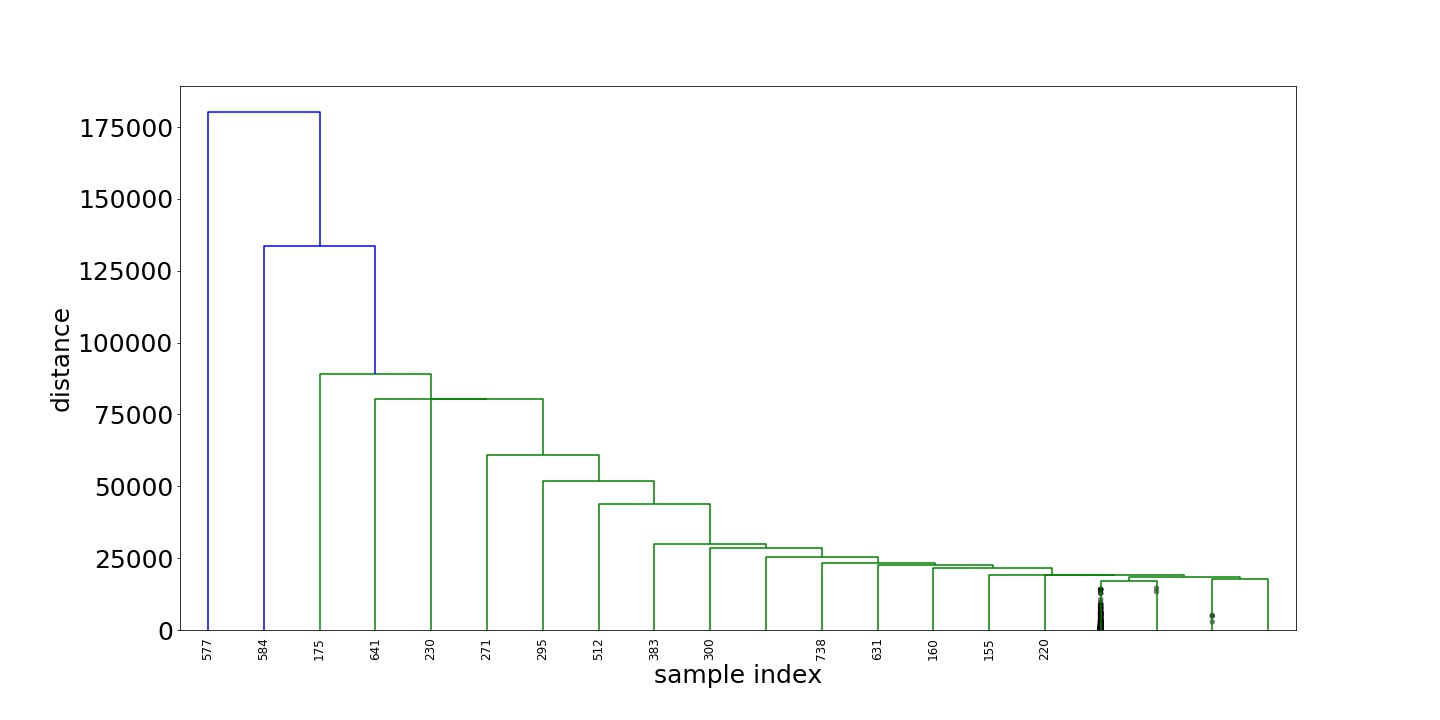
\includegraphics[width=\linewidth]{chapter3/figure/dendogram.jpg}
	\caption{Hierarchical Clustering Dendrogram (truncated to the last 20 merged clusters)}
	\label{fig:dendogram}
\end{figure}

In order to select the optimal number of clusters, we plotted the knee-elbow figure (\ref{fig:kneeelbow}). It shows the variation of WSS (within cluster sum of squares) and BSS (between cluster sum of squares) as the number of clusters increase.\\

\begin{figure} [htp!]
	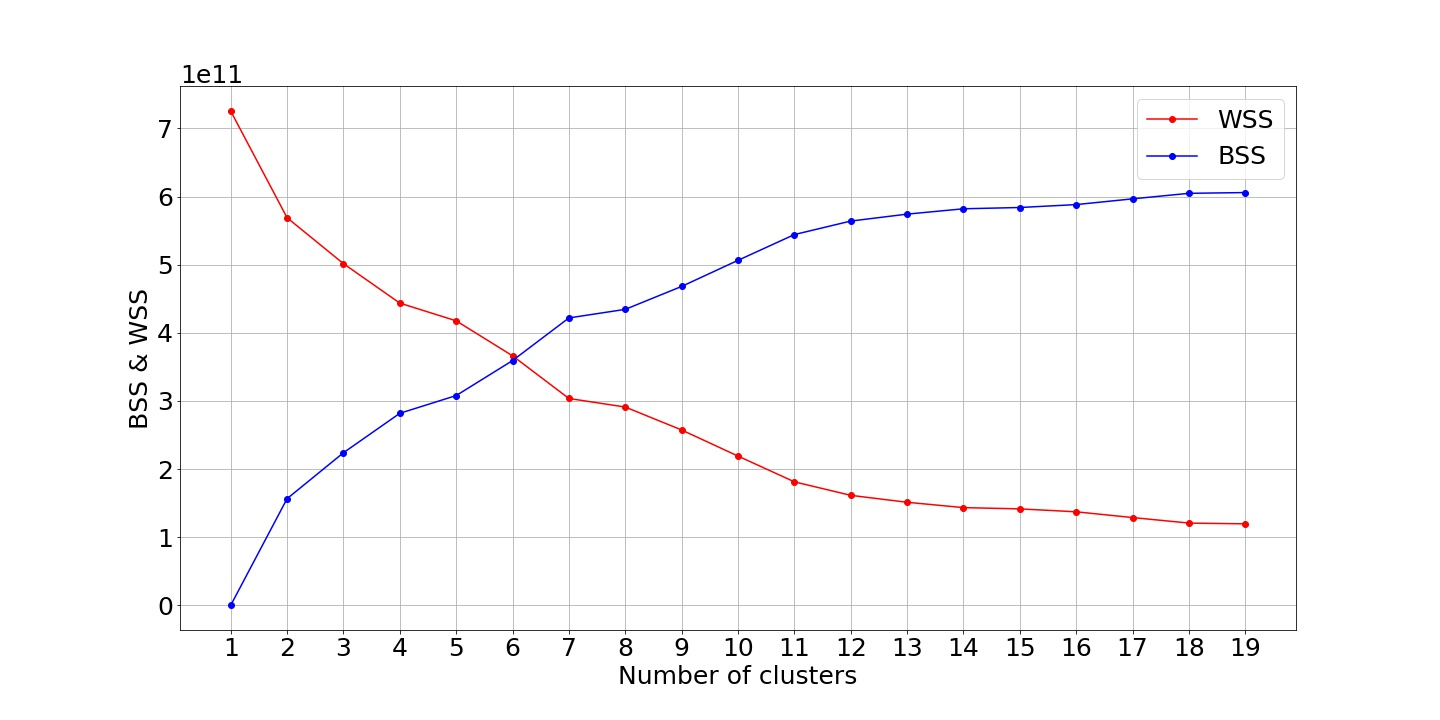
\includegraphics[width=\linewidth]{chapter3/figure/kneeelbow.jpg}
	\caption{Hierarchical Clustering - knee-elbow}
	\label{fig:kneeelbow}
\end{figure}

It is clear that there are no well-defined elbows or knees, both curves seems to be "smooth", so it were hard to pick a reasonable k (number of clusters) for the algorithms to come.

Then we tried another approach. We applied the \emph{K-means} algorithm and we plotted the elbow methond (\ref{fig:elbow}). In this figure there is an elbow beetween k=3 and k=4, so the most accurate solution were represented by four clusters.

\begin{figure}
	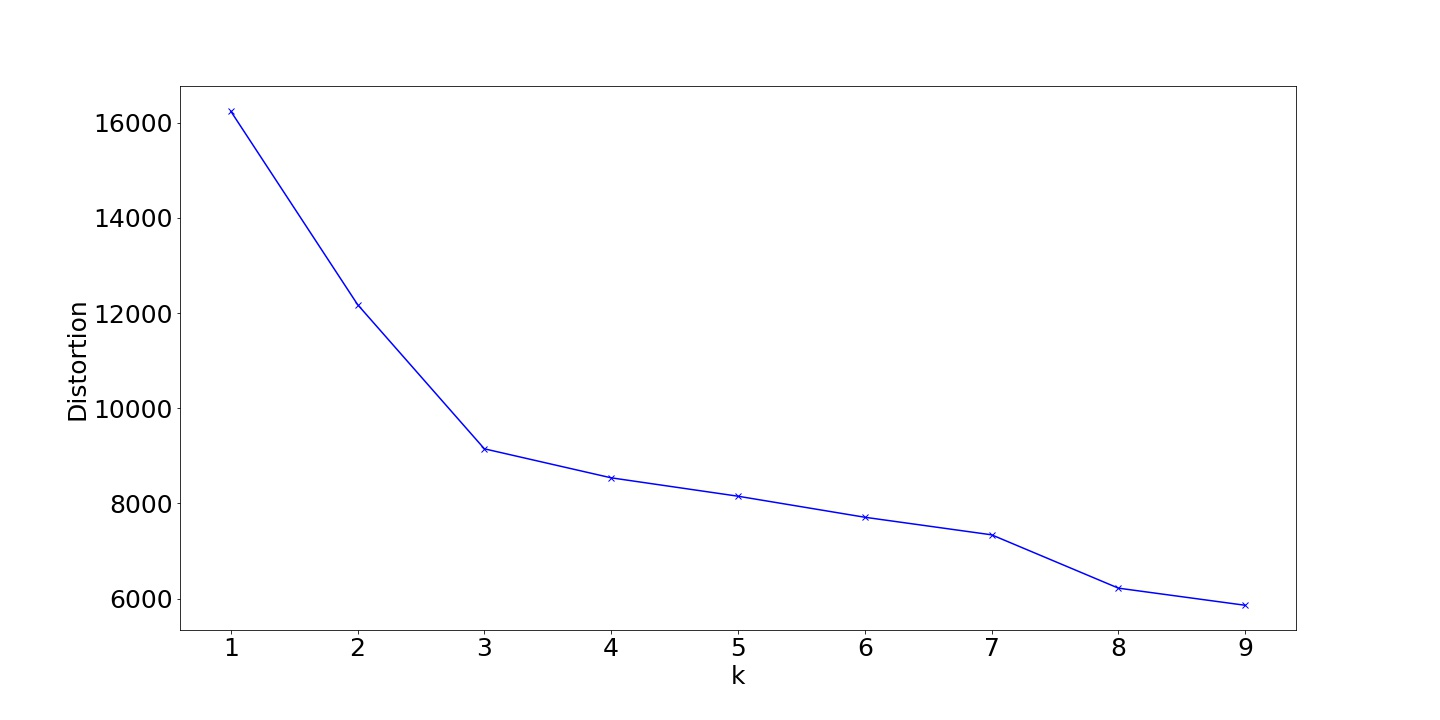
\includegraphics[width=\linewidth]{chapter3/figure/elbow.jpg}
	\caption{The Elbow Method showing the optimal k}
	\label{fig:elbow}
\end{figure}

As this process came to an end, we manually inspected the resulting clusters.

\begin{center}
	\begin{tabular}{ll}
	\\cluster&size\\
	\hline\hline
	cluster 1&82\\
	cluster 2&648\\
	cluster 3&2\\
	cluster 4&16\\\hline
	\end{tabular}
\end{center}

Cluster 2 contains most of the samples, while the others have fewer elements.
We observed the Twitter profile of all the elements belonging to cluster 1, 3, 4 and a small sample of profiles for cluster 2.

Unfortunately there was no correlation among accounts in the same cluster, so this technique didn't seem to fit the speeding up of the labeling process, nor to create useful features for a classifier.

\section{Collection}
\label{sec:dataset}
The clustering approach did not help us, but the manual inspection of the clusters allowed us to get in touch with some existing bots, making us understand which categories of bots are most common on the social network. In particular we detected 4 main classes:
\begin{itemize}
	\item[\PencilRight]NSFW bots
	\item[\PencilRight]News-spreader
	\item[\PencilRight]Spambots
	\item[\PencilRight]Fake-followers
\end{itemize}

We started with a hand-labeling of the Varol dataset \cite{Varol}. For each account we analyzed its profile and tweets and we assigned it a label according to the categories we identified.  We have faced some unexpected behaviors among bot accounts, that didn't fit the above-mentioned categories. In these cases, tehy were temporarily signed as "general purpose".

We also found genuine users, who we thought that had been incorrectly added to the dataset.
This task culminated with the collection of the following bots:

\begin{center}
	\begin{tabular}{ll}
		\\category&labeled account\\
		\hline\hline
		NSFW&31\\
		news-spreader&71\\
		spambots&418\\
		fake-followers&5\\
		general purpose&63\\
		genuine&104\\\hline\\		
	\end{tabular}
\end{center}

\emph{"General purpose"} accounts are sometimes bots with no goal, they aim to emulate human behavior and often they were recognizable just because their description informs other users about their own nature.

Sixtythree users were not enough to represent a class and it was not possible to find a large list of those accounts who act like them, so we added all these ids to the "genuine" group. Even if this choise brought some noise to our data, that allowed us to provide our data more heterogeneity.

\emph{"NSFW"} accounts are only thirtyone elements, anyway the problem of pornography is a known issue on Twitter. In \cite{Varol} they clusterize users too. "These bot clusters exhibit some prominent properties: cluster C0, for example, consists of legit-looking accounts that are promoting themselves (recruiters, porn actresses, etc.)" \cite{Varol}.
This kind of users are often banned by Twitter, so it is likely that the accounts that we were not able to scrape, used to belong to this category.
Therefore we firmly believed that obtaining further accounts of this class was fundamental.

Finally it is clear that even fake-followers were few, since they were not considered in the Varol research, but they are important in \cite{Cresci}, so we decided to expand this category too.

All these samples were not enough to train a classifier, hence we needed to collect more data. We perform this task by focusing on one category at a time.

\subsection{NSFW}
\emph{Not safe for work} is a tag used on internet to mark all that URLs, web pages, e-mails that contain nudity, intense sexuality, profanity or violence. In particular we wanted to collect a specific sub-category: the pornbots. In order to collect them, we used the BotBlock dataset.

BotBlock contains thousands of pornbot ids. We wanted to gather about 6000 samples, an amount that would have been enough for the final dataset, with regards to its balance.
Since they were sorted according to their creation date, we shuffled the whole list. Then, using the Twitter API, we looked for accounts that weren't deleted yet. 
We needed to scrape profile features and tweets, so we couldn't consider banned accounts. The user list was initially shuffled to allow us to collect users with different ages. This emerged as a very useful setp, because we gathered both more long-lived accounts and more extreme accounts (which probably have shorter lives). We finally obtained 6903 users and 198378 tweets.
\subsection{News-spreader}
Many bots on Twitter are news-spreader. The goal of these users is to spread politics, sports or actuality news. Often their behavior is not harmful, they just retweet statuses from newspapers accounts. However, there are users created to diffuse fake news. In the last few years Twitter has been used to boost politics propaganda. During elections or political campaigns, ad hoc accounts are created to divulgate specific political idea.

As a recent study highlighted, about the 80\% of these "pre-elections bots" are still alive \cite{Disinformation}. We think that part of our news-spreader dataset includes some of those accounts.

We started gathering these ids by exploring Hoaxy.
We used two different approaches.
\begin{figure}
	\centering
	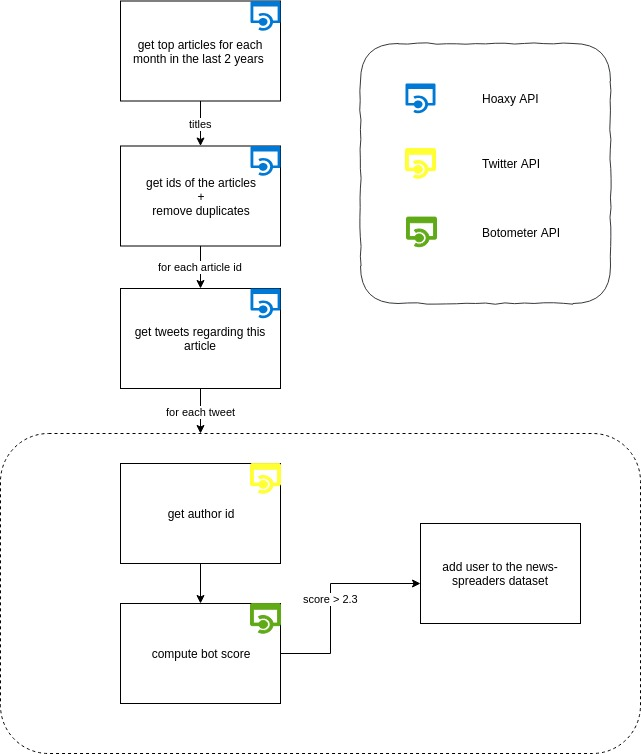
\includegraphics[width=250px]{chapter3/figure/news-spreader.jpg}
	\caption{Collection of news-spreading bots, approach 1}
	\label{fig:news-spreaders}
\end{figure}
The first way (in figure \ref{fig:news-spreaders}) consisted in collecting the twenty top popular fake news, for each month, in the last two years. We performed this task using the Hoaxy APIs. Thanks to this service, we obtained all the tweet ids that have spread the considered claim. With the official Twitter APIs we collected all the users involved in this spreading activity. We finally passed all these accounts to the Botometer API, since many of the retrieved users were humans.

We set a threshold, in order to classify a user as a bot. That threshold is 2.3 due to the willing of including some false positives in our data, increasing the heterogeneity in their behaviors and the challenge level for the classifiers. We think that a high intra-homogeneity among classes could lead the models to perform well on the training data, but worse over unseen ones.

The second approach just consisted in collecting the most popular news-spreaders according to Hoaxy. In consistency with the mentioned threshold, profiles with a Botometer score lower then 2.3 were still discarded.

Finally we checked every profile added to this dataset and removed all that users who didn't tweet enough statuses to be included in this class. This hand-made analisys made us know that there are no bots who only spread fake-news. Usually they tweet a lot of verified news and some fake ones, to keep their credibility.
We reached 3590 accounts and 333699 tweets.

\subsection{Spam-bots}
As seen before, spambots were already collected in \cite{Cresci}. Authors allowed us to access to their dataset, so we obtained the spambots list by sampling their data. Due to homogeneity reasons, we needed to perform scraping again, since we needed different features compared to the available ones.
We selected users from:
\begin{itemize}
	\item[\PencilRight]traditional spambots 1
	\item[\PencilRight]social spambots 2
	\item[\PencilRight]social spambots 3
\end{itemize}

We chose this categories because they contain the most popular kinds of spambots, that are the ones who advertise products, services or mobile applications. We ignored \emph{"social spambots 1"}, since they are italian news-spreaders and \emph{"traditional spambots 3 and 4"}, since we retrieved enough job-offer spammers during the hand-made labeling. If we had stored too many bots of this category, we would not have been able to generalize on generic spambots. Finally we gathered 4943 accounts and 458809 tweets.

\subsection{Fake-followers}
The collection of this class was quite easy. We initially performed scraping of the data collected by the Cresci research \cite{Cresci}. Many of these accounts had already been banned, so we could not collect their features. In order to enrich our dataset, we created a new Twitter account (figure \ref{fig:dibebot}). Then we bought fake followers from two different services:
\begin{itemize}
	\item[\PencilRight] instakipci.com/
	\item[\PencilRight] rantic.com/buy-legit-twitter-followers/
\end{itemize}

\emph{Instakipci} provides low-quality followers. Usually they have no tweets, no followers and a they have a lot of followings.

\emph{Rantic}, on the other hand, ensures more realistic followers. They seem to have a real network of friends and, sometimes, they tweet too.

By using both services, we gathered a more miscellaneous dataset.
We collected 6307 users and 41683 tweets.
\begin{figure}
	\centering
	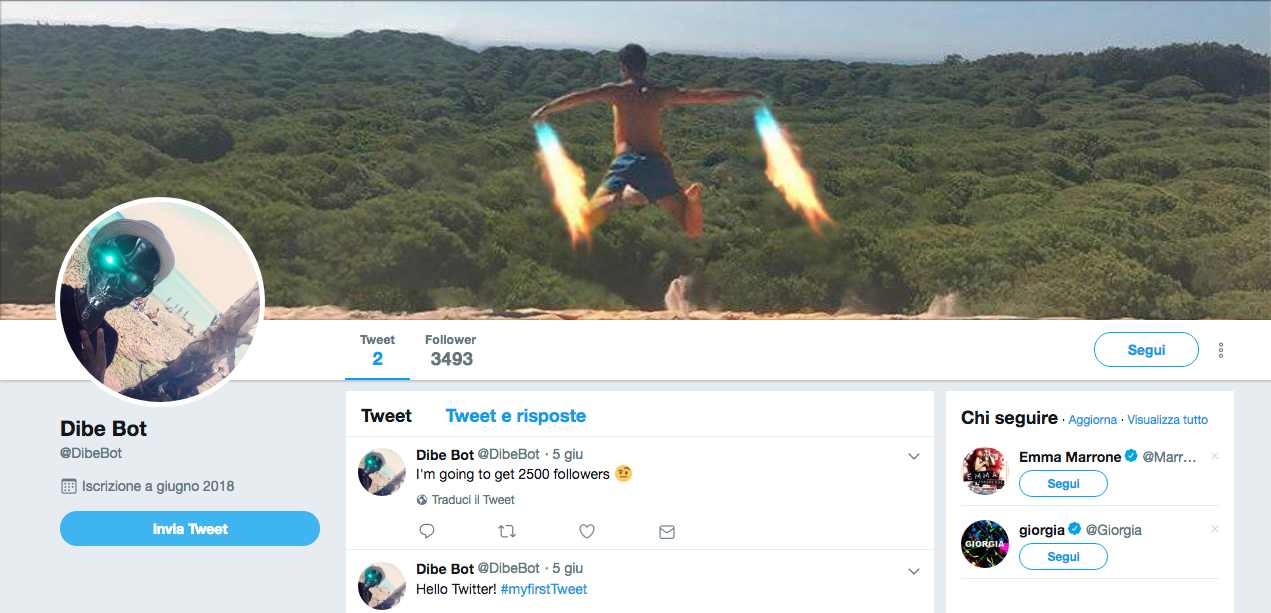
\includegraphics[width=\columnwidth]{chapter3/figure/dibebot.png}
	\caption{Collection of fake-followers bots}
	\label{fig:dibebot}
\end{figure}

\subsection{Genuine}
Finally we needed genuine accounts. We used again the Cresci dataset \cite{Cresci} and we filled it with all the Varol users labeled as humans. We again performed scraping on the existing accounts and we collected 3661 users and 263240 tweets in total.

\newpage

\section{Data visualization}
As the collection of the data was completed, we explored our final dataset.
A first look (\ref{fig:bubble}) shows us how many user accounts we collected (y axis) for each class and how many tweets we could scrape (diameter). It is easy to observe that fake-followers and nsfw bots have less tweets than the others,while news-spreaders have a lot of tweets, but we collected less profiles.
\begin{center}
	\begin{tabular}{ll}
		\\category&target id\\
		\hline\hline
		NSFW&0\\
		news-spreader&1\\
		spambots&2\\
		fake-followers&3\\
		general purpose&4\\\hline\\		
	\end{tabular}
\end{center}


\begin{figure}[htp!]
	\centering
	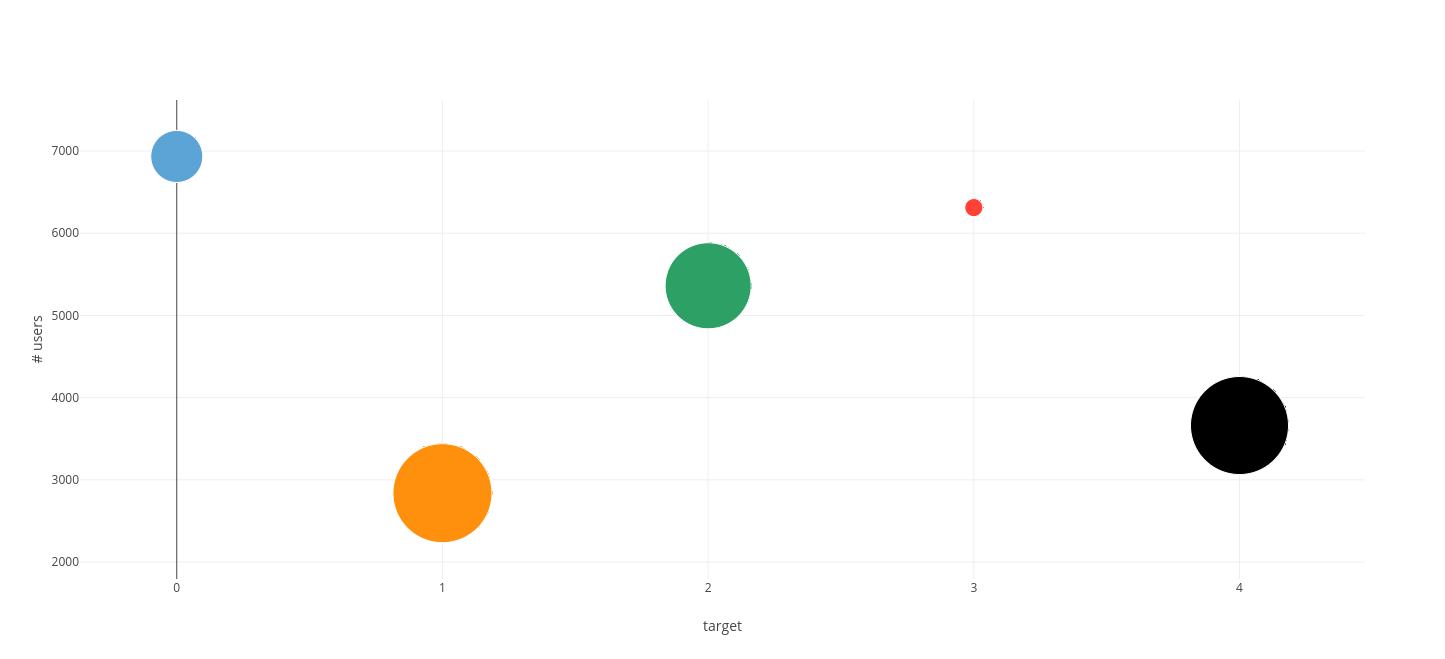
\includegraphics[width=\columnwidth]{chapter3/figure/bubble.png}
	\caption{users amount and tweets}
	\label{fig:bubble}
\end{figure}

Then we plotted the heatmap of the correlation matrix (\ref{fig:heatmap}). We wanted to undestand if some feature was more usefull to predict the correct target. This plot suggested us that there were no feature highly correlated to the target.
\begin{figure}
	\centering
	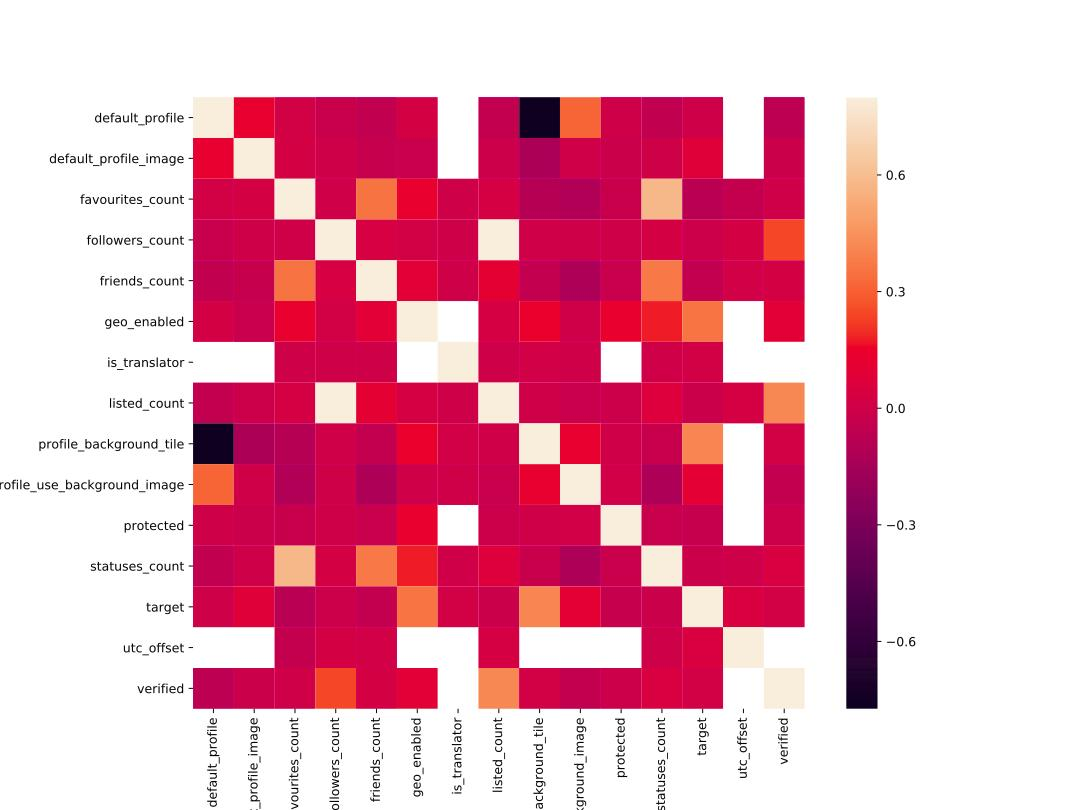
\includegraphics[width=\columnwidth]{chapter3/figure/heatmap.jpg}
	\caption{heatmap}
	\label{fig:heatmap}
\end{figure}

Moreover in figure (\ref{fig:msno}) it is possible to see the distribution of the missing values. This is fundamental for the features engineering step.

\begin{figure}
	\centering
	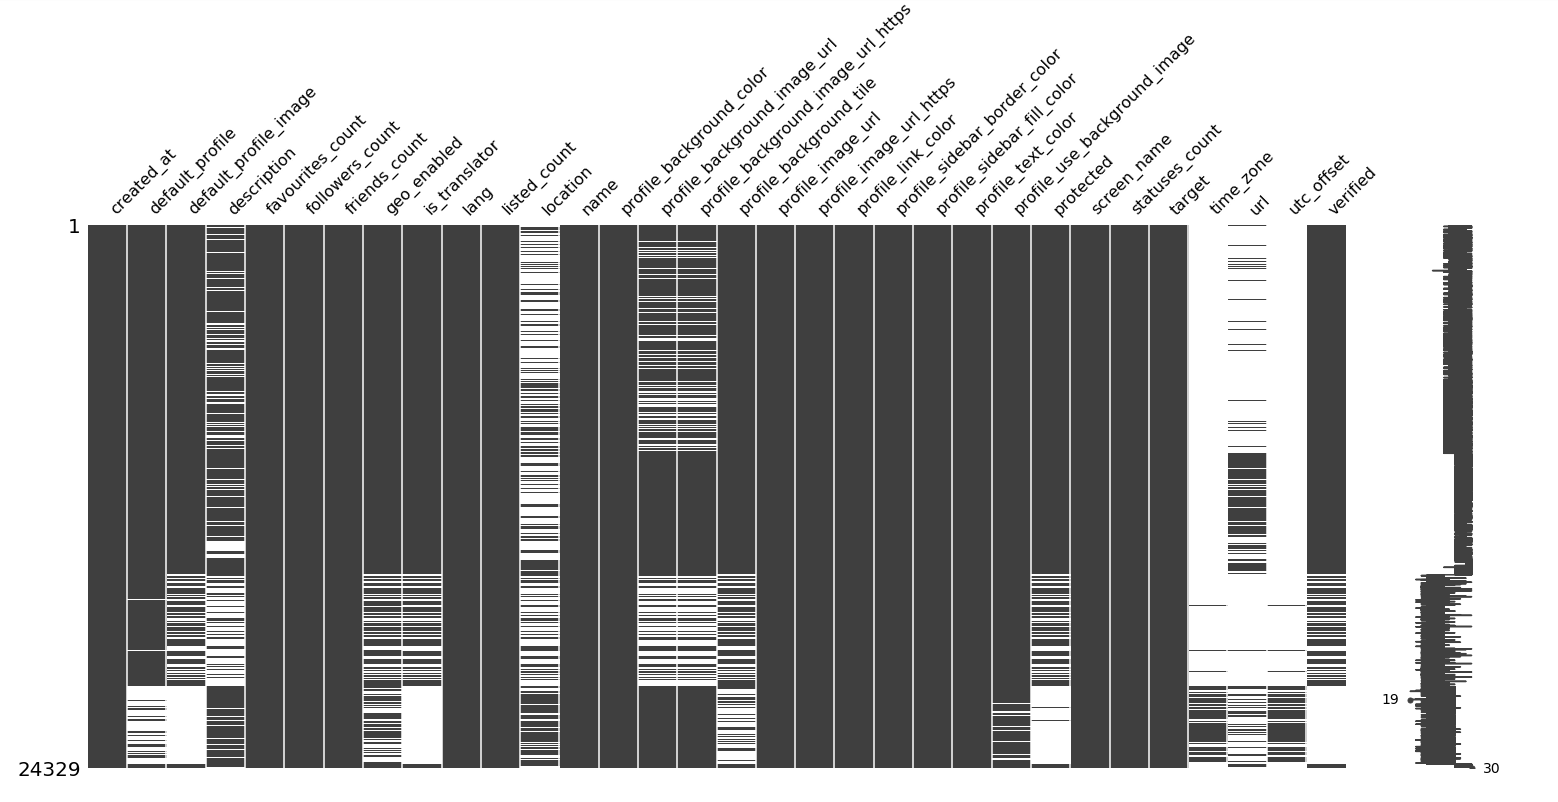
\includegraphics[width=\columnwidth]{chapter3/figure/msno.png}
	\caption{heatmap}
	\label{fig:msno}
\end{figure}

\newpage
Finally we performed three further analisys. With the heatmap we could not detect which features were more important. Anyway,during the hand-labeling step, we understood that some of these features were instead very usefull to identify a few classes of our dataset. These attributes are \emph{"followers\_count"}, \emph{"friends\_count"} and \emph{"statuses\_count"}. For each of them we plotted a boxplot. It is a method used to represent groups of numerical data through their quartiles. In Figure \ref{fig:box_statuses} we can analyze the statuses count for each target. We collected up to 100 tweets for each user, so this chart is limited to 100. Here we can notice an interesting behavior: \emph{"news-spreaders"} and \emph{"spambots"} are the classes with more tweets, while \emph{"fake-followers"} have less statuses. By reflecting on the gols of the bots, this result is exactly what we expected to see. In fact \emph{"fake-followers"} don't need to tweet, they just need to exist, while other types of bots have to publish many statuses, to draw attention on their contents.

\begin{figure}
	\centering
	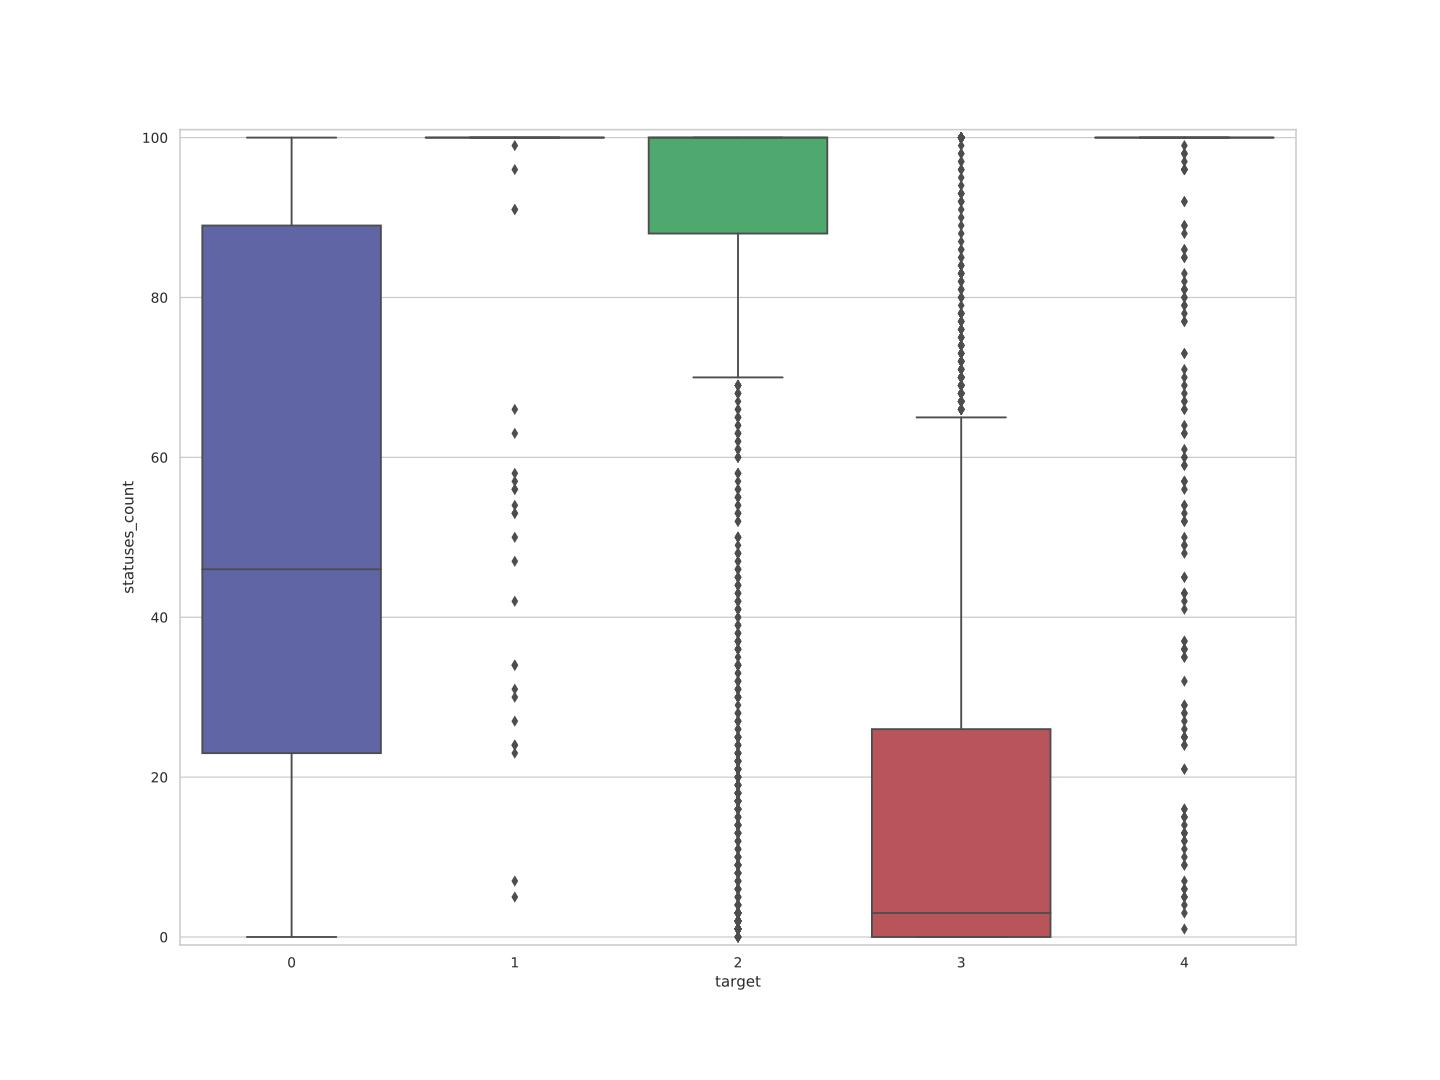
\includegraphics[width=\columnwidth]{chapter3/figure/boxplot_statuses.jpg}
	\caption{boxplot statuses\_count}
	\label{fig:box_statuses}
\end{figure}
\newpage

\begin{figure}
	\centering
	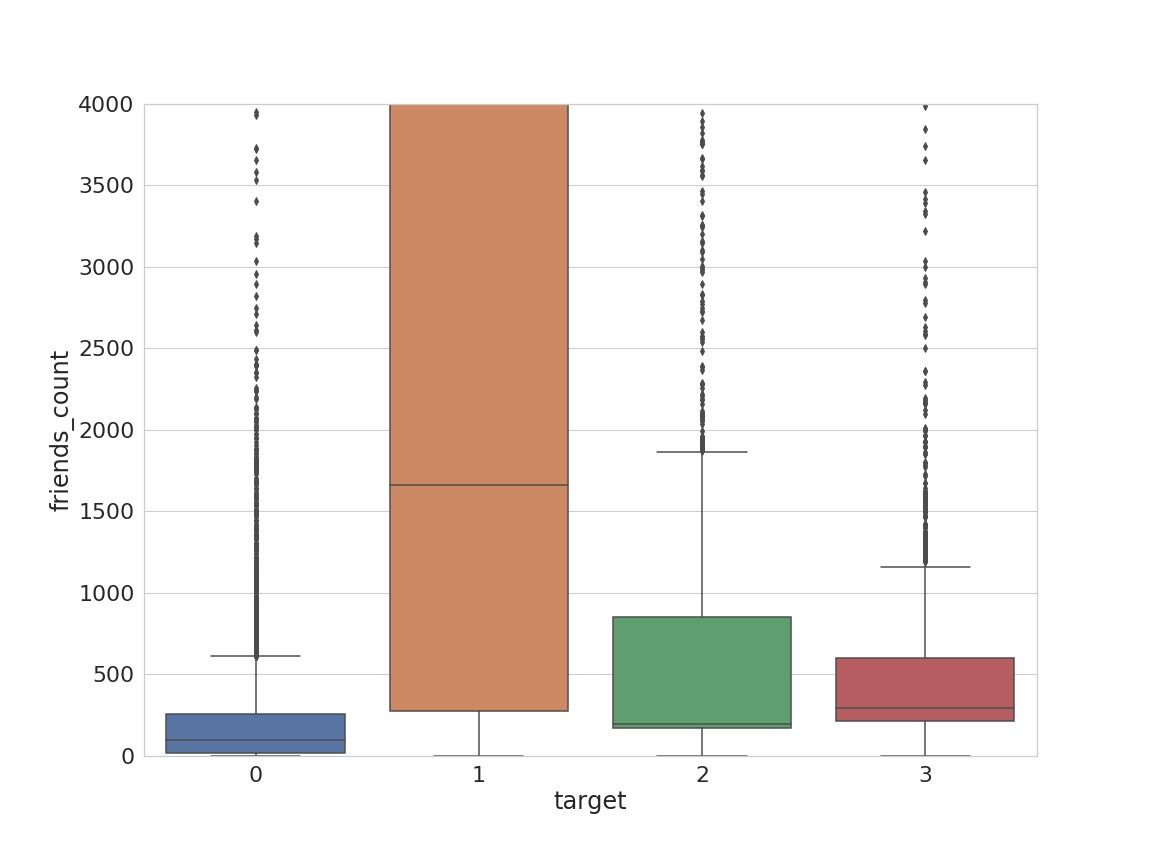
\includegraphics[width=\columnwidth]{chapter3/figure/boxplot_friends.jpg}
	\caption{boxplot friends\_count}
	\label{fig:box_friends}
\end{figure}

\begin{figure}
	\centering
	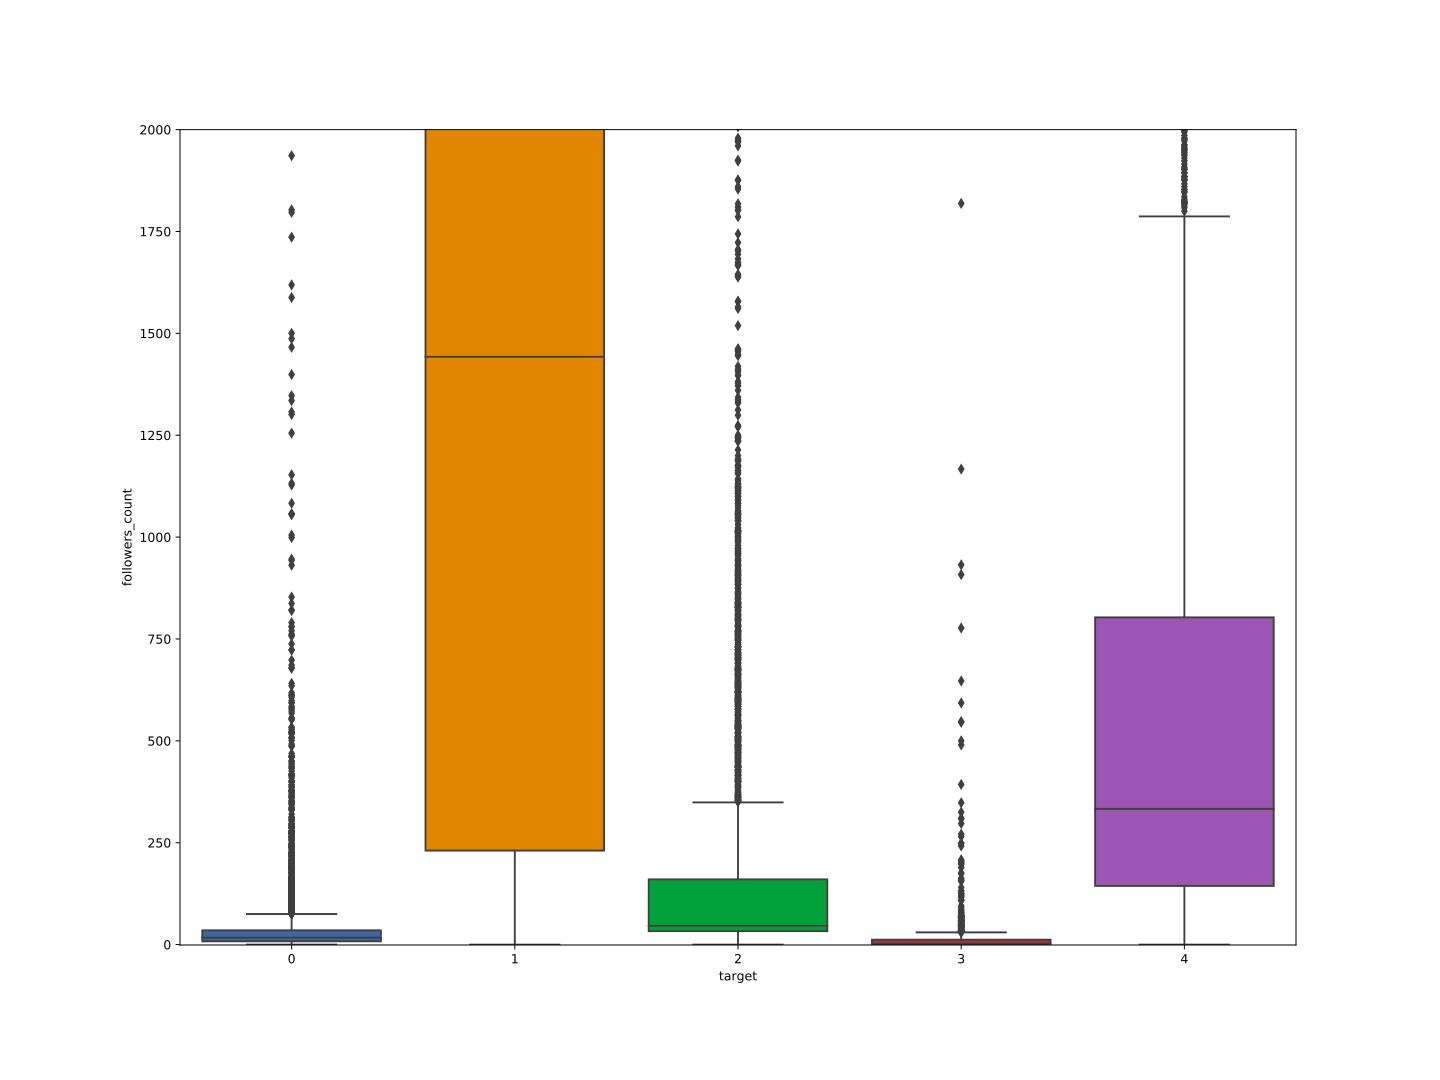
\includegraphics[width=\columnwidth]{chapter3/figure/boxplot_followers.jpg}
	\caption{boxplot followers\_count}
	\label{fig:box_followers}
\end{figure}
In Figure \ref{fig:box_friends} and \ref{fig:box_followers} we performed the same analisys considering the \emph{"friends\_count"} and \emph{"followers\_count"} features. We limited the charts to 4000 and 2000 to keep them understandable. This two figures show us that \emph{"news-spreaders"} usually have a bigger network, while \emph{"fake-followers"} just follow few users. \emph{"News-spreaders"} network may depends on the popularity of the news media. Other categories are more balanced and their differences can be attributed to the data and not to a different behavior between them. For the genuine accounts we need to make an extra observation. Of course there are a lot of human users on Twitter and they have very different behaviours. In our dataset we included profiles with an average popularity (\ref{fig:box_followers}), so they are neither VIPs nor fresh users without followers. Furthermore they have a smaller network of friends (\ref{fig:box_friends}), which is in the average of the other categories. Finally they actively use twitter (\ref{fig:box_statuses}) since we were able to collect about 100 tweets for each of them. 